%%% use twocolumn and 10pt options with the asme2e format
\documentclass[twocolumn,10pt]{asme2ej}
\newcommand{\gbf}[1] {\mbox{\boldmath${#1}$\unboldmath}}
\newcommand{\R}{\hbox{I \kern -.5em R}}
\usepackage{epsfig}
\usepackage{graphicx}
\usepackage{epstopdf}
\usepackage{color}
\usepackage{wrapfig}
\usepackage[hidelinks]{hyperref}
\usepackage{subfigure}
\usepackage{amsmath}
\usepackage{url}
\urlstyle{same}
\usepackage{algorithm}
\usepackage[noend]{algpseudocode}
\usepackage{caption}
\usepackage[font=small]{caption}
\usepackage{algorithmicx}


\hypersetup{
  colorlinks   = true, %Colours links instead of ugly boxes
  urlcolor     = blue, %Colour for external hyperlinks
  linkcolor    = blue, %Colour of internal links
  citecolor   = blue %Colour of citations
}

\newcommand{\nothing}{}
\newcommand{\req}[1]{(\ref{#1})}
\newcommand{\pos}[1]{\stackrel{+}{#1} \! }
\newcommand{\half}[1]{\frac{#1}{2}}
\newcommand{\nhalf}[1]{(\frac{#1}{2})}
\newcommand{\singleline}{\baselineskip 0pt}
\newcommand{\expo}[1]{exp$({\bf {#1}})$}

% for displaying argmin command
\DeclareMathOperator*{\argminA}{arg\,min}

\def \Pluckerian{Pl\"uckerian }
\def \Plucker{Pl\"ucker }
\def \plucker{Pl\"ucker}
\def \Bezier{B\'{e}zier }
\def \BEZIER{B\'{E}ZIER }
\def \Shrocker{Schr\ddot{o}cker}

%\title{Linkage Synthesis for defect free path and motion generation.}
\title{Data Driven Defect Free Synthesis of Planar Mechanisms for Path and Motion Generation}
%%% first author
\author{Shrinath Deshpande, Anurag Purwar\footnote{Corresponding Author}\\
    \affiliation{
    Computer-Aided Design and Innovation Lab \\
    Department of Mechanical Engineering\\
    Stony Brook University\\
    Stony Brook, New York, 11794-2300
    }
   }

\begin{document}
\maketitle

\begin{abstract}
\end{abstract}

%%%%%%%%%%%%%%%%%%%%%%%%%%%%%%%%%%%%%%%%%%%%%%%%%%%%%%%%%%%%%%%%%%%%%%
\section{Introduction}
Classic mechanism synthesis problem deals with computing type and dimensions of linkage system for performing specific tasks, which are categorized as path, motion and function generation.
This problem has been dealt with many approaches with the aim of finding acceptable solutions for practical situations.
In spite of increasing applications of electronically controlled manipulators, single degree freedom mechanical linkages will still important.
This is justified by new areas of application opened by technologies like nanotechnology, bio-mechatronics.
Therefore mechanisms theory will retain its position in the research community.

The motion and path generation problems are exhaustively researched topics.
Several text books, such McCarthy and Soh \cite{sohmccarthy}, Sandor and Erdman~\cite{Sandor}, Hunt \cite{Hunt78}, Hartenberg and Denavit \cite{Hartenberg},  Suh and Radcliffe \cite{Suh78}, and Lohse \cite{lohse2013} cover the science and art of planar four-bar and higher-order linkages.
The majority of these theories dont account for circuit and branch defect in synthesized mechanisms, which can render these mechanisms useless for practical applications.
The defects in mechanisms are thoroghly discussed in Chase and Mirth\cite{chase}.
Few of the approaches have taken branching defect into account. Their literature goes here ->->

Original contribution of this paper is in 1) a data driven framework that solves this problem using database look up, followed fine tuning via local optimization,
2) objective function and a \emph{signature} of coupler curves invariant under similarity transformation.
The invariant signature of coupler curves reduces solution space by a major fraction, which is further subjected to dimensionality reduction using Auto-encoder Neural Networks.
Clustering is performed on compresed latent representation of encoder to create the database hierarchy.
When a inputs a motion or a path, a query representing invariant signature of the input is raised for k nearest neighbors among cluster centers in the database.
The neighbor is defined as trajectory whose part or whole has a similar signature to input. These k neighbors are then subjected to find fine tuning to obtain set of solutions.

\section{Invariant Representation of Coupler Motion}
A coupler motion is a continuous trajectory in SE2 space, for path generation problem we ignore the orientation aspect of it.
In order to farmulate signature of the coupler motion which is invariant under similarity transform, we detach orientation information from path at the first step.
This is done because orientation does not suffers from the similarity operations.
We use formulations developed by Cui et.al\cite{cui2009} for open 2D curve matching, and build the signature of planar rigid body motion.

\subsection{Cubic B-Spline Fitting}
The discrete version coupler path is fitted with cubic b-splines with a approximate curvature parameterization such that more points will be sampled at the locations where curvature changes are higher. BSpline knot vector parameterization is given by,
\begin{equation}\label{u_1}
  u_i = u_{(i-1)} + \sqrt{{(x-\bar{x})}^2 + {(y-\bar{y})}^2}
\end{equation}
 where $(\bar{x}$, $\bar{y})$ is center of the bounding box sample points. We further normalize knot-vector $u$ to keep it between 0 and 1.

Figure~\ref{bsplineFitting} presents a comparison of B-spline fittings to path given with different timing information. It can be seen that B-spline samples more points where radius of curvature is small.

\begin{figure}
\centering
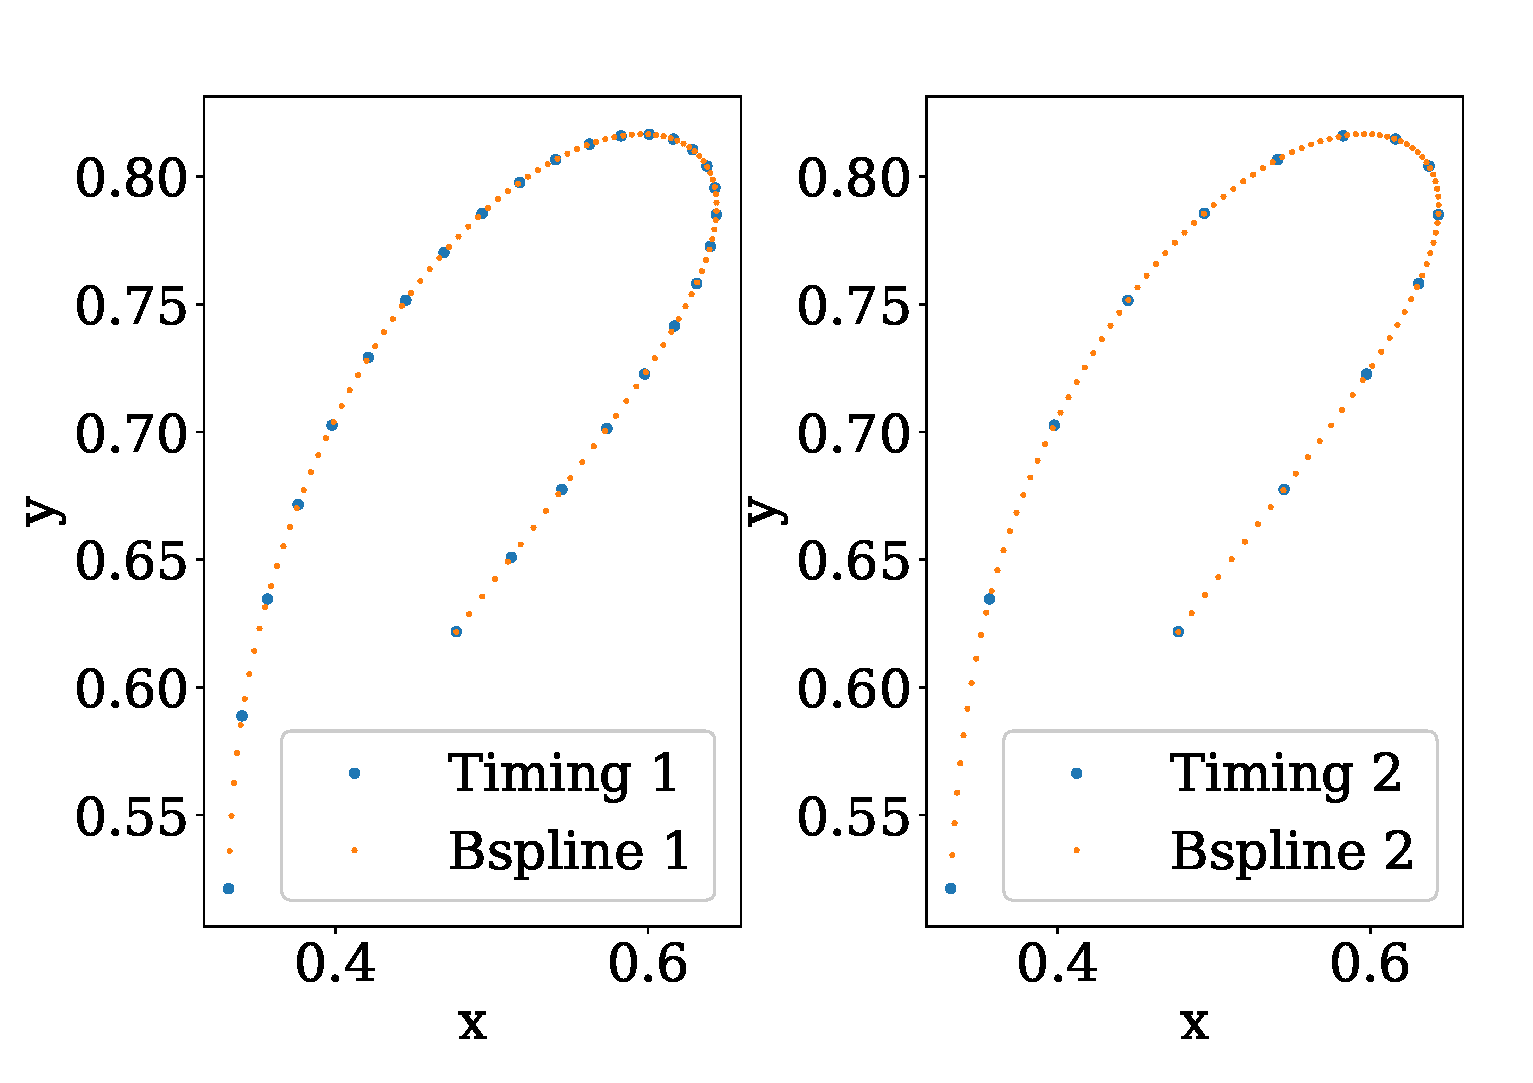
\includegraphics[width=240pt]{figure/fig_bspline.eps}
\caption{Cubic B-spline with curvature parameterization on the same curve with two different sampling rates.}
\label{bsplineFitting}
\end{figure}

\subsection{Curvature and Integral of Curvature Computation}
The curvature ($k$) at arc length $s$ and its unsigned integral upto $s$ are respectively given by,
\begin{eqnarray}
  k(s) = {\ddot{\textbf{x}}}(s), \\
  K(s) = \int^{s}_0 |k(s)|, \\
\end{eqnarray}

where ${\textbf{x}}: (x(s), y(s)$.

Figure~\ref{curvatureK} shows computed curvatures and its unsinged integral of coupler trajectory shown in Fig.~\ref{bsplineFitting}.

\begin{figure}
\centering
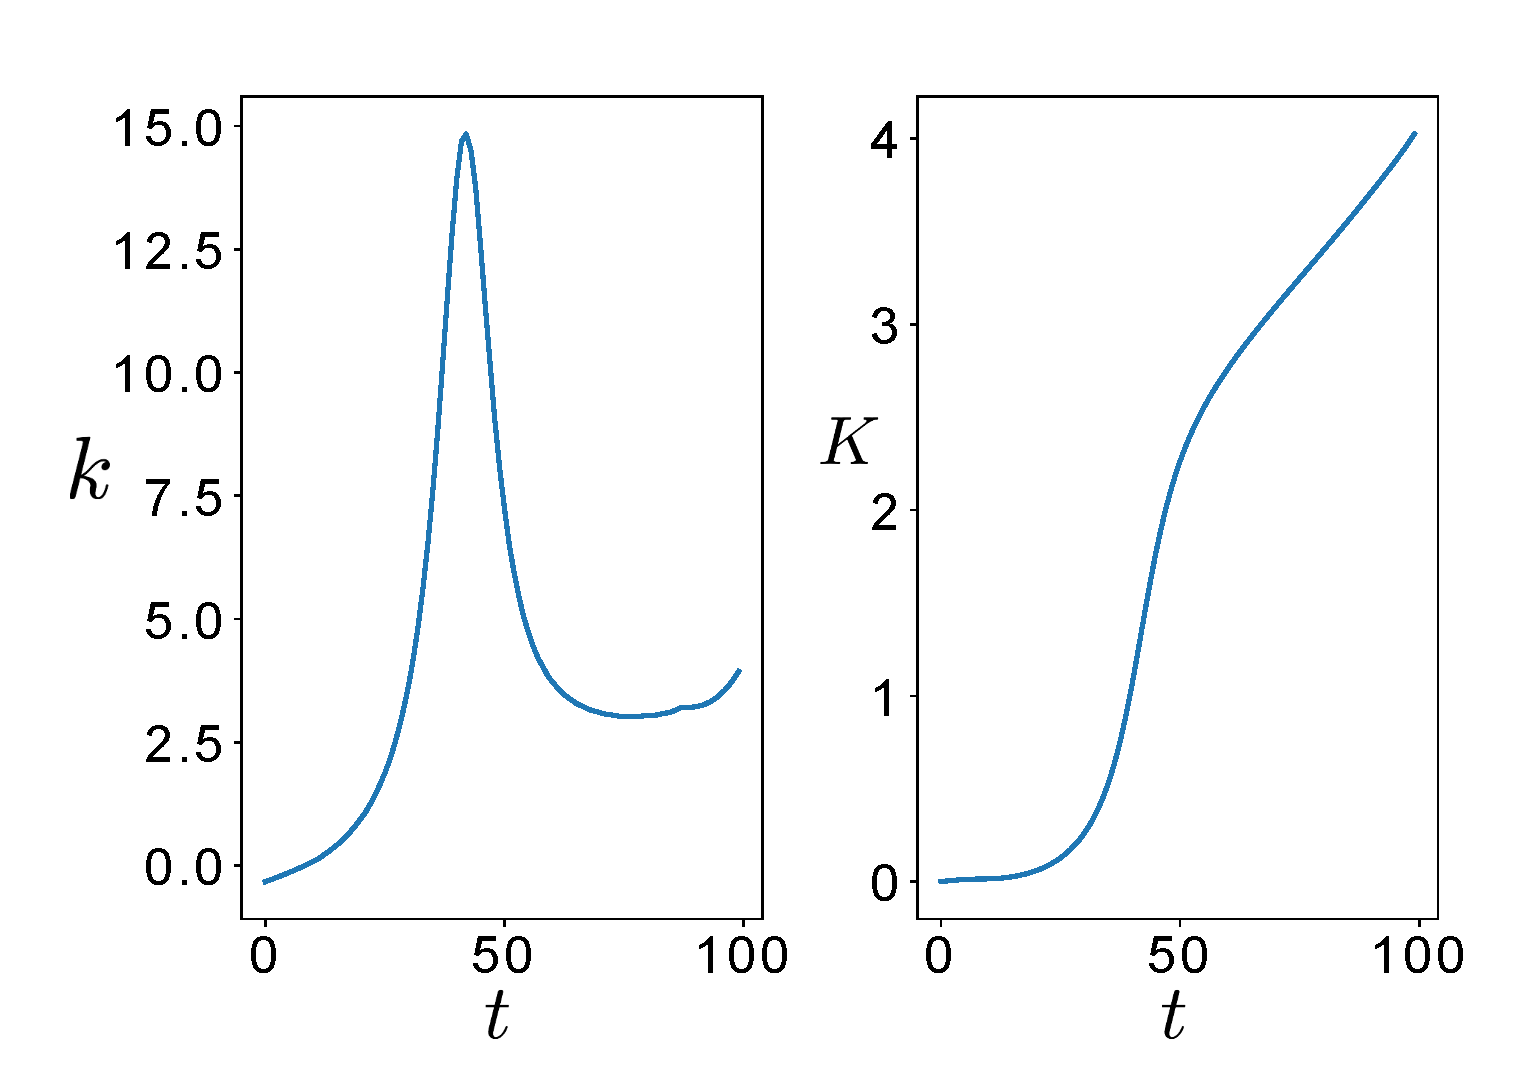
\includegraphics[width=240pt]{figure/fig_curvatureK.eps}
  \caption{arc length parameterized Curvature and Integral of curvature for the path shown in Fig.~\ref{bsplineFitting} with timing 1.}
\label{curvatureK}
\end{figure}

\subsection{Signature}
Now we re-sample the curvature at equal intervals of $K(s)$.
This is done by fitting a BSpline curve through curvature plot, with choosing know vector $u_{2}$ as given by,
\begin{equation}\label{u_2}
  u_i = u_{(i-1)} + {(K_i-K_{(i-1)})}
\end{equation}

Now plotting re-sampled $k$ vs $K$ gives us the signature of the coupler path. This signature is invariant under similarity transformation; for proof see\cite{cui2009}.
Figure~\ref{signature} shows the path from Fig.~\ref{bsplineFitting} with two different timings and their corresponding signatures.
It can be seen that timing has a negligible effect on signatures.
The minor distortions is due to small difference in the shape of fitted B-Spline.

\begin{figure}
\centering
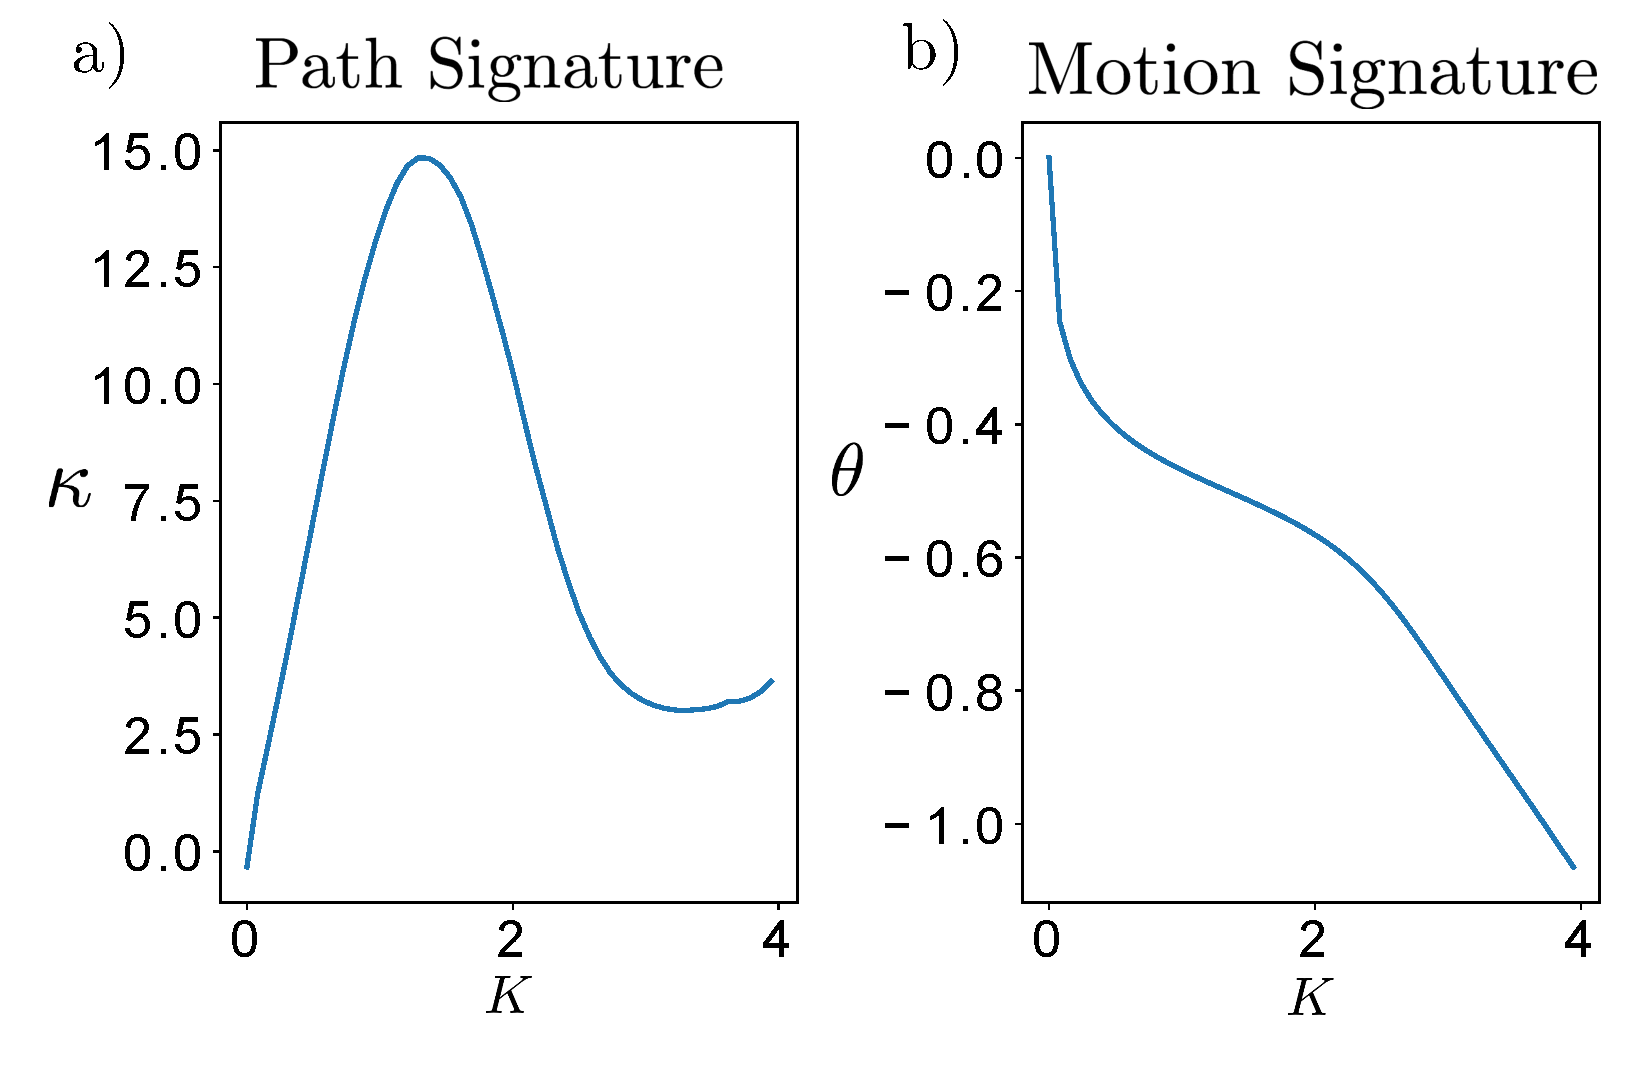
\includegraphics[width=240pt]{figure/fig_signatures.eps}
  \caption{Signatures of the path with two different timings from Fig.\ref{bsplineFitting}. It can be seen that signatures have minimal sensitivity towards change in timing of the input.}
\label{signature}
\end{figure}

\subsection{Partial Matching of Coupler Curves}\label{sec_ncc}
The signatures can be used for partial matching using normalized cross-correlation\cite{cui2009}.
Normalized cross-correlation function $(C_n)$ is a convolution operation between two signals (or curve signatures) $F(i)$ and $t(i)$ given by,

\begin{equation}
  Cn(j) = \sum_{i}^{t_{span}} \frac{(F(i+j) - \bar{F}_{t_{span}})(t(i) - \bar{t})}{\sqrt{\sum_{i}^{t_{span}}{(F(i+j) - \bar{F}_{t_{span}})}^2\sum_{i}^{t_{span}}{(t(i) - \bar{t})}^2}}
\end{equation}

Where $Cn(j)$ is the normalized cross-correlation value when template $t(i)$ is matched to $F$ at $j^{th}$ index. Here $t(i)$ acts as template that tries to find best match against $F(i)$ while sliding over it along j.
Domain of $Cn(j)$ is [-1, 1], where 1 represents the complete match.
Maximum score of the matching represents similarity of the template in F, and location at which maximum occurs is the start point.
Figure~\ref{ncc} depicts normalized cross correlation function over the sliding domain $j$ for two curves shown in Fig.~\ref{wholePart} where the second curve is a part of first curve modified by scaling and translation.

\begin{figure}
\centering
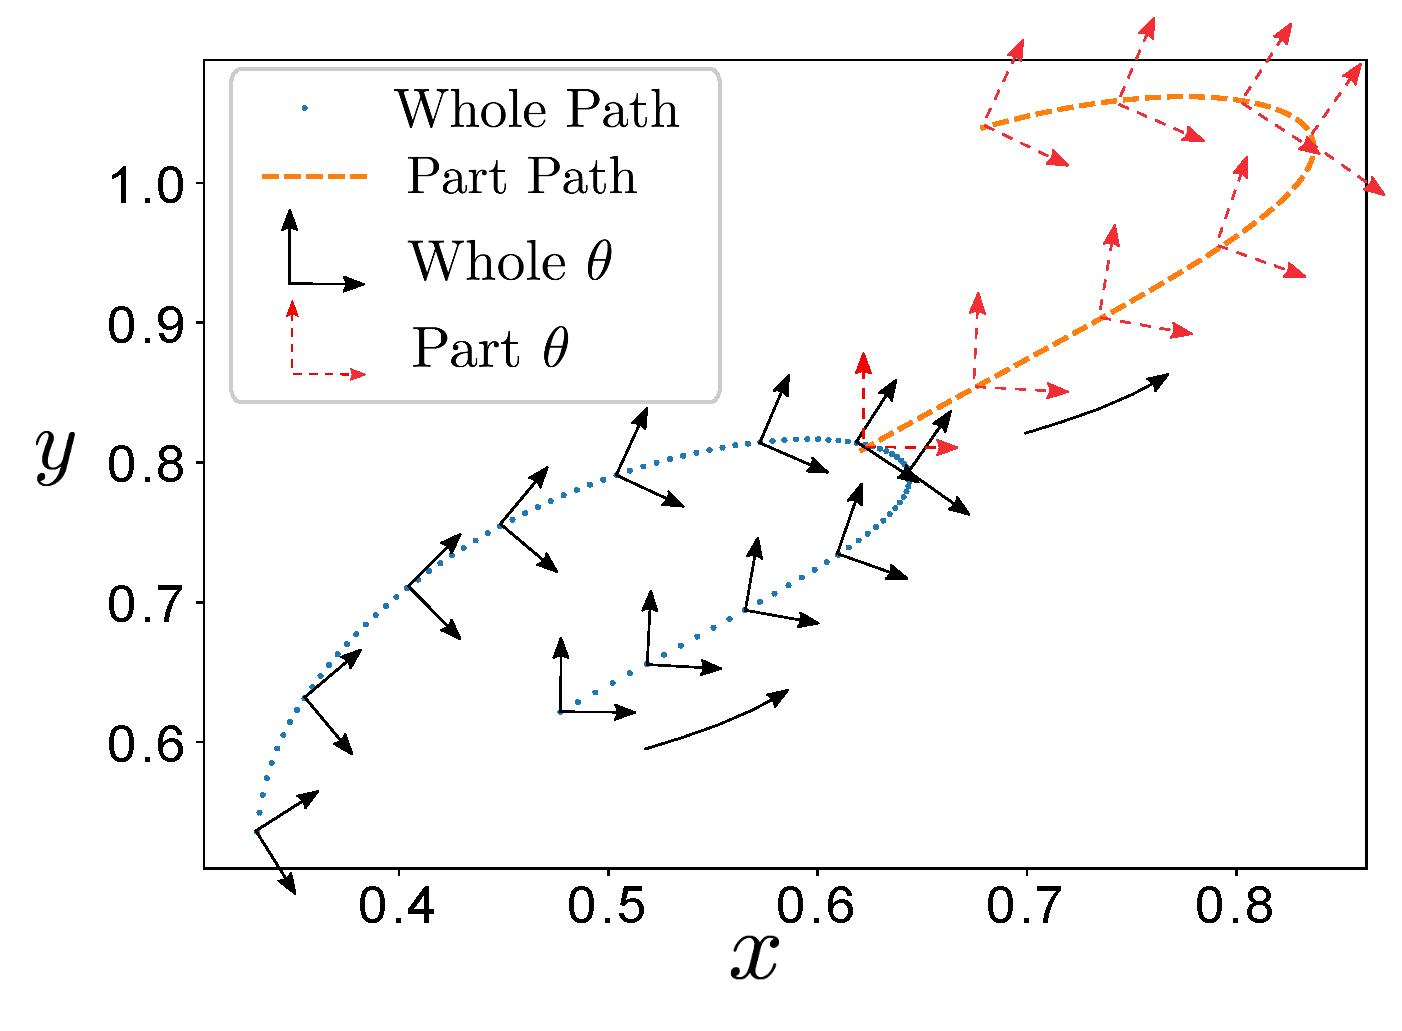
\includegraphics[width=240pt]{figure/fig_whole_part.eps}
  \caption{Part path is formed by trimming whole path followed by translation and scaling.}
\label{wholePart}
\end{figure}

\begin{figure}
\centering
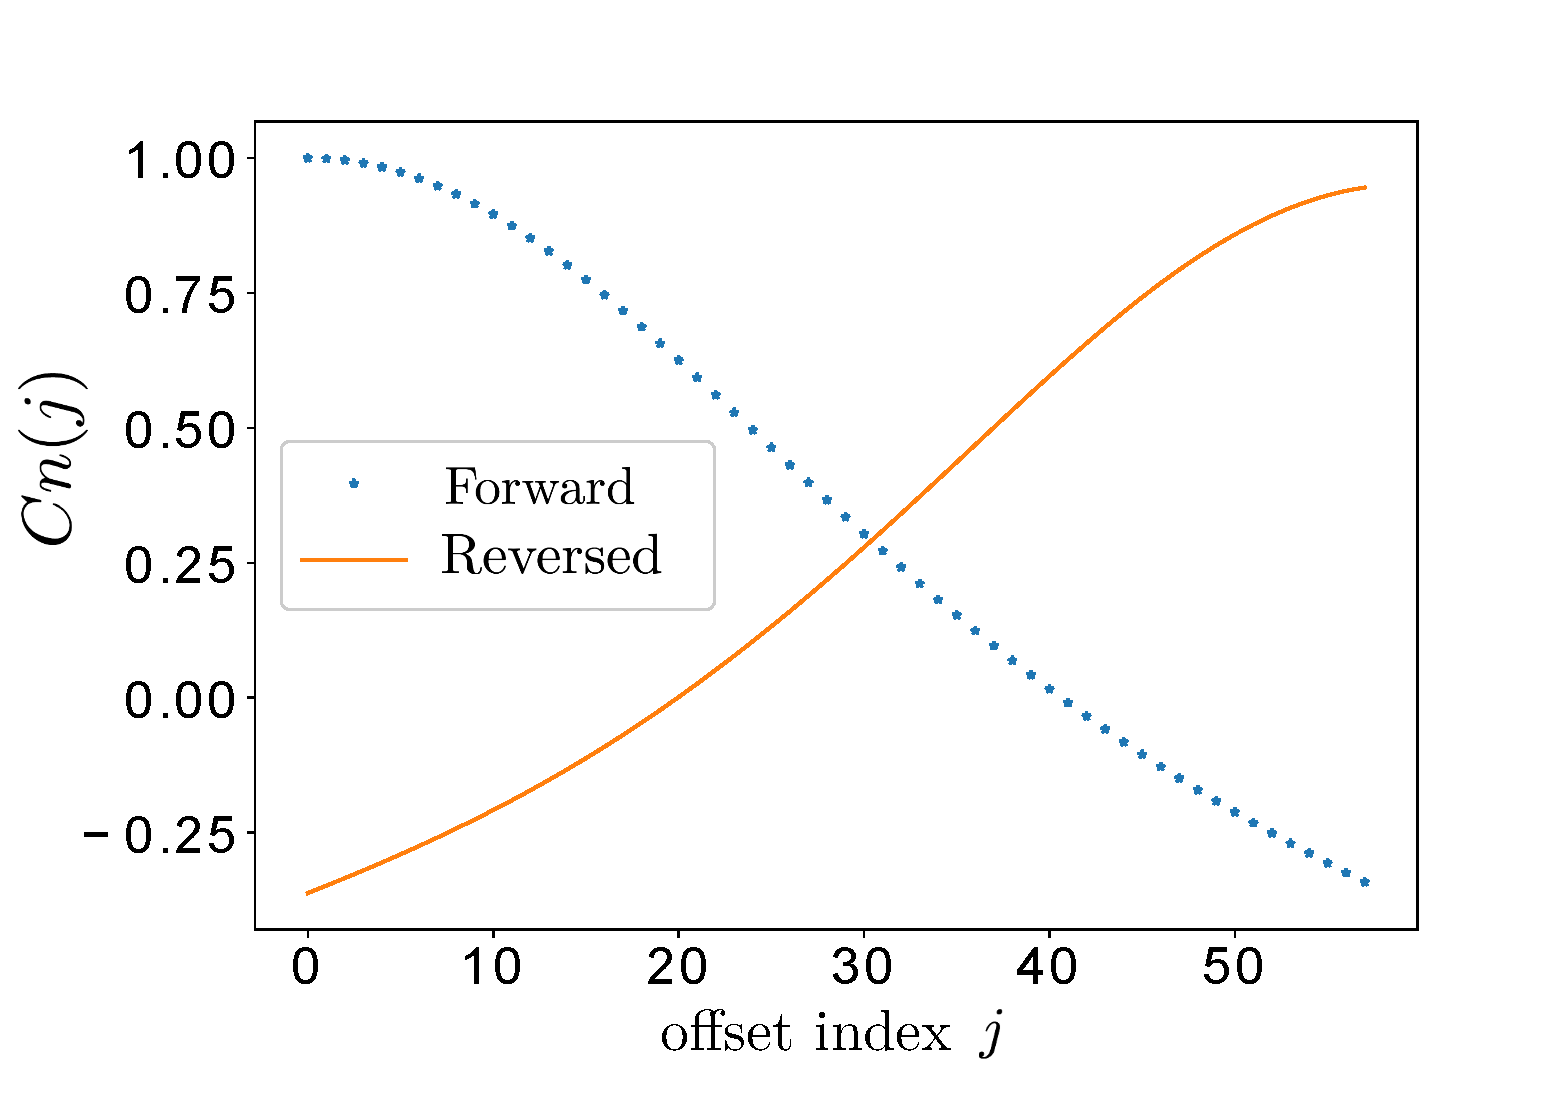
\includegraphics[width=240pt]{figure/fig_ncc.eps}
  \caption{Normalized cross correlation of the signatures is shown. It can be seen that exact match is found at $j=0$.}
\label{ncc}
\end{figure}

\subsection{Signature of coupler motion}\label{sec_sign}
Now that we have a invariant representation of path, we can formulate signature of coupler motion.
First we subtract initial angle from rest of the curve.
Next step is to fit a B-spline through coupler angles using the same knot vectors given in~\req{u_1}, followed by r-esampling at parameters given by~\req{u_2}.
The obtained orientation data plotted against $K$ results into motion signature of the trajectory as shown in fig.~\ref{motionSignature}

\begin{figure}
\centering
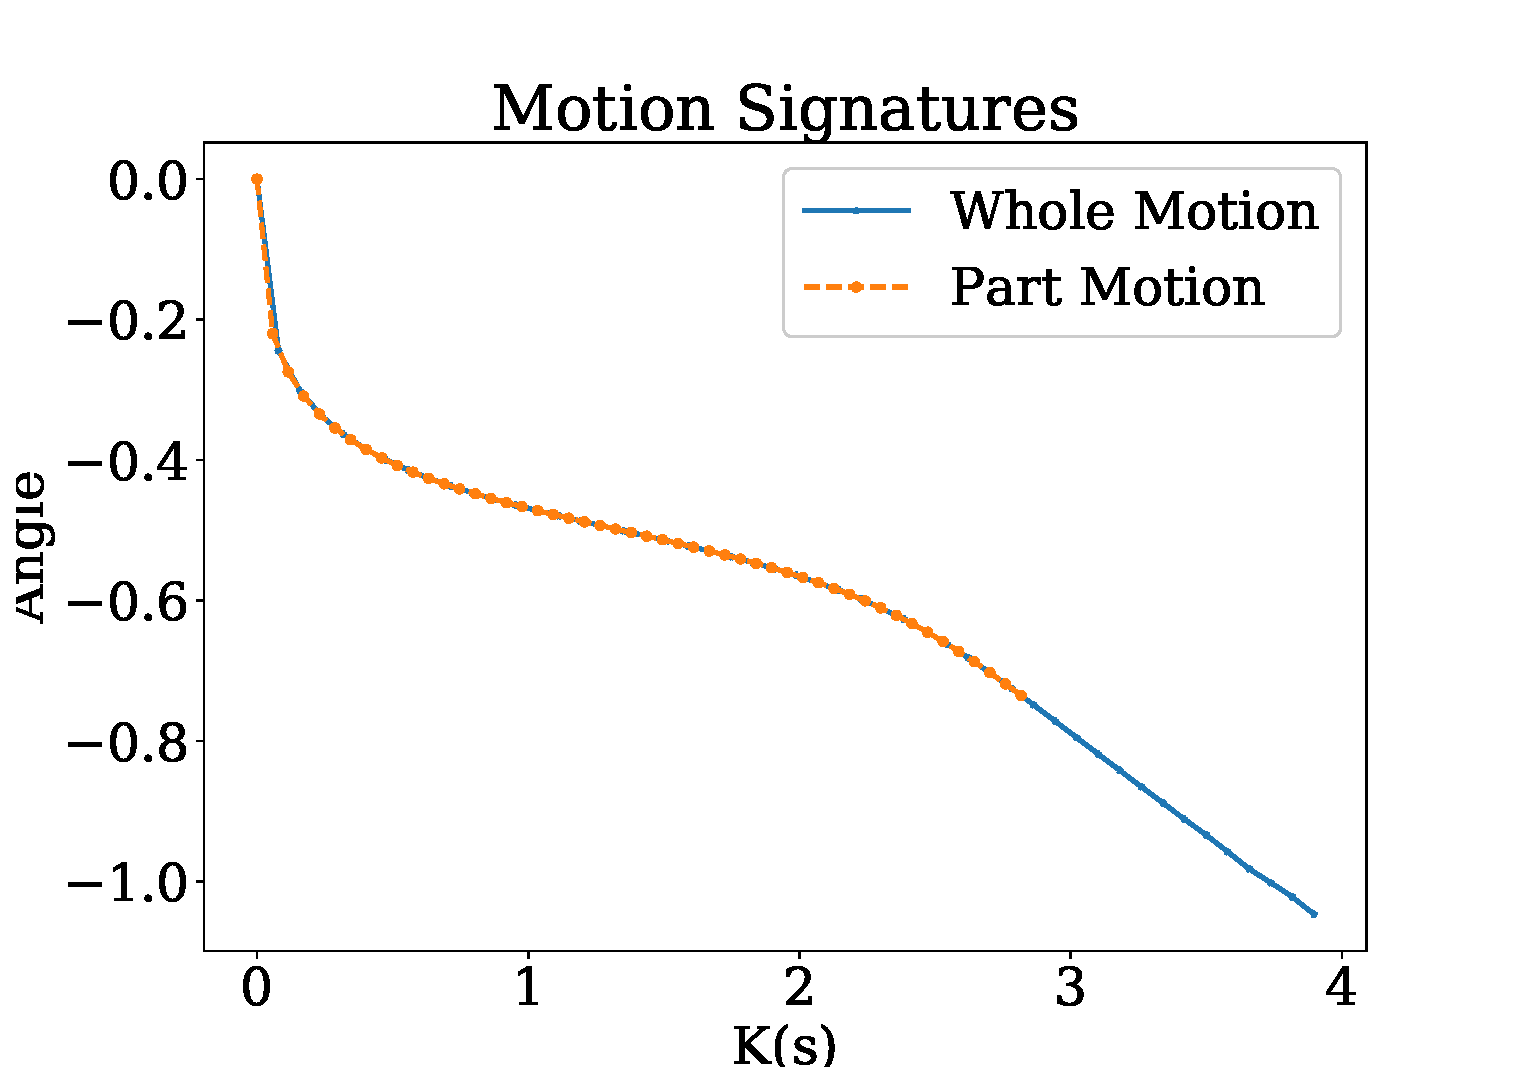
\includegraphics[width=240pt]{figure/fig_motion_signatures.eps}
  \caption{Motion Signatures of the trajectories shown in Fig.\ref{wholePart}. The same correlation function can be used to compute whole-to-part matching.}
\label{motionSignature}
\end{figure}

\subsection{Objective Function for Synthesis}
The Normalized Cross-Correlation function presented in the section~\ref{sec_ncc} can be used the criterion for motion (or path) synthesis of any planar linkage, where the objective is to find a linkage, that produces a motion whose part or whole corresponds to target motion (or path).
Thus we can formulate the optimization problem given by,

\begin{equation}\label{objectiveFun}
  \argminA_{\textbf{\emph{l}}} f_{obj}(\textbf{\emph{l}}) = 1 - \max\limits_{j}(Cn(j))
\end{equation}
where $\textbf{\emph{l}}$ is the vector of linkage parameters for perticular planar linkage.
In case of four-bar, $\textbf{\emph{l}}: l_1, l_2, l_3, l_4, l_5$, with $l_i$ is link ratio of $i^{th}$ link shown in Fig~\ref{fourbar}.

\begin{figure}
\centering
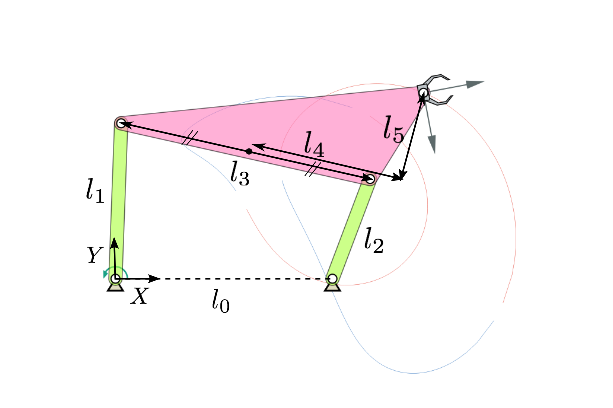
\includegraphics[width=240pt]{figure/fig_fourbar.eps}
  \caption{Parametric representation of four-bar linkage with all revolute joints.}
\label{fourbar}
\end{figure}

Objective function evaluation step consists of calculation of coupler motion and finding its best normalized cross-correlation score.
It is important to note that representation obtained in Section~\ref{sec_sign} reduces size of the linkage parameters in optimization.
This optimization problem can be solved using search methods which do not require gradient computation as algebraic representation of objective function in terms of linkage parameters is not possible.
We can employ global optimization methods such as differential evolution, simulated annealing at the start and local optimization methods link powell's method towards the end for faster convergence\cite{ullah1997}.
Section~\ref{examples} presents results for various optimization techniques used.

Considering highly non-linear nature of the problem, finding a good initial guess proves to be game changing.
Thus we exploit the advantages of data driven approach for finding many good initial guesses or if get lucky, the solution itself.

\section{Sensitivity Analysis of Signatures}
Owing to the complex relationship between parameter space and generated motion, small change in linkage parameters can produce large and discontinuous structural change in the generated motions.
For example small change in crank length can open a previously close loop.
Most of the analytical methods like Fourier analysis can not capture the continuity at such singular locations, which adversely affect the optimization process.
In contrast to this behavior, Signatures derived in Sec.~\ref{sec_sign} has smooth transition at these singular locations.
To make our point, we perform Sensitivity Analysis as follows:
A four-bar with link ratios ($l_1:0.3$, $l_2:1$, $l_3:1.5$, $l_4:1$, $l_5:1$) is subjected to gradual change in parameter $l_1$ in the range (0.3, 0.8) in steps of 0.1.
Figure~\ref{saCouplerCurves} shows coupler motion of the fourbars associated with change in $l_1$.
Although the close circuit breaks to form open curves, It is evident how smooth the shape changes in the process.
This smoothness is captured in the Heat Map shown in Fig.~\ref{saHeatmap} obtained by similarity evaluations via Normalized Cross-Correlation of corresponding signatures.
If we construct the graph (see Fig.~\ref{saGraph}) based on the adjacency matrix and igore the edges when distance is more than 0.2, we get a \emph{small world network}\cite{watts1998}.

\begin{figure}
\centering
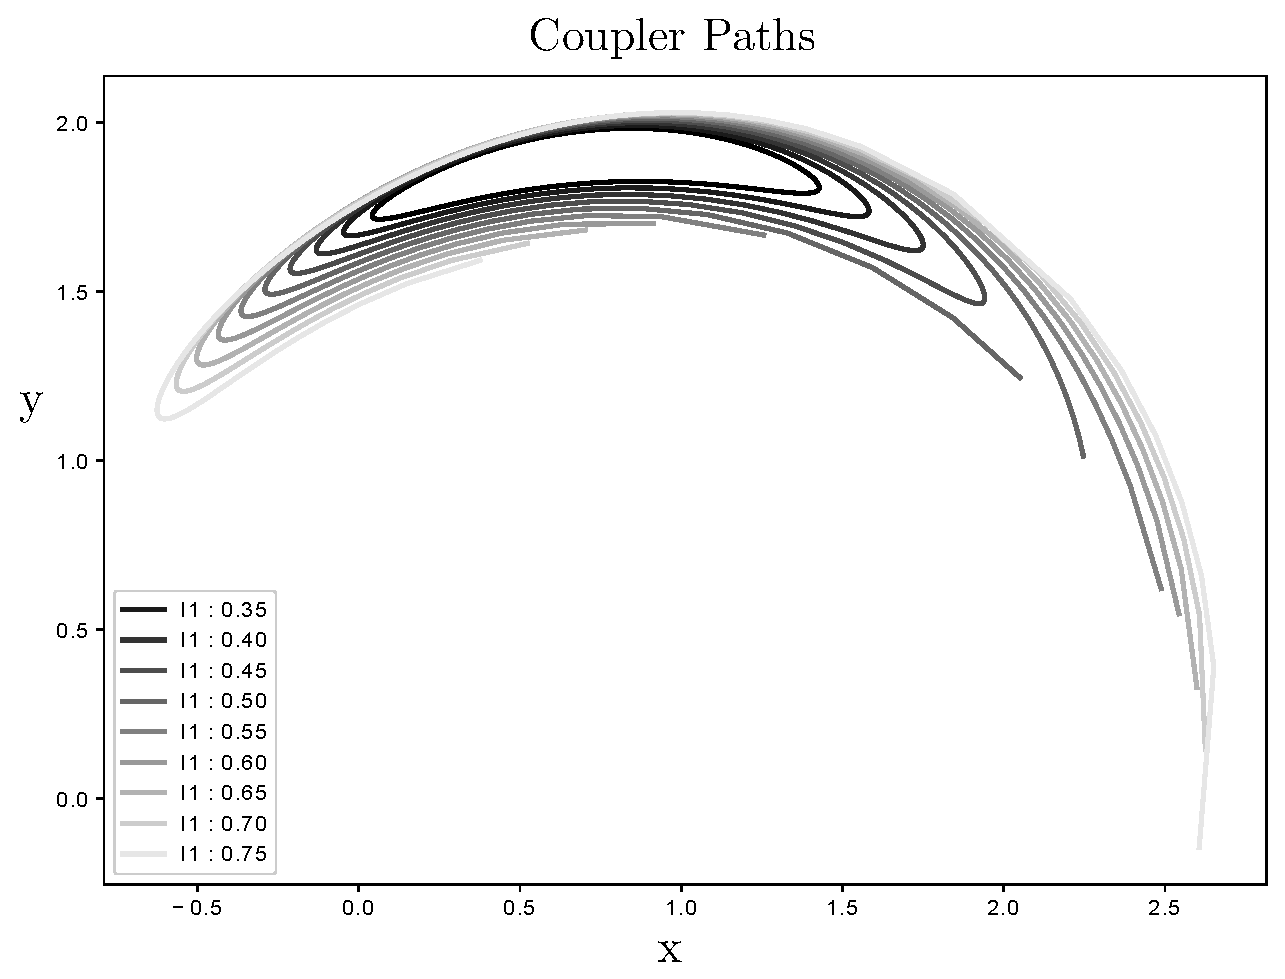
\includegraphics[width=240pt]{figure/fig_sa_coupler_curves.eps}
  \caption{Hi}
\label{saCouplerCurves}
\end{figure}

\begin{figure}
\centering
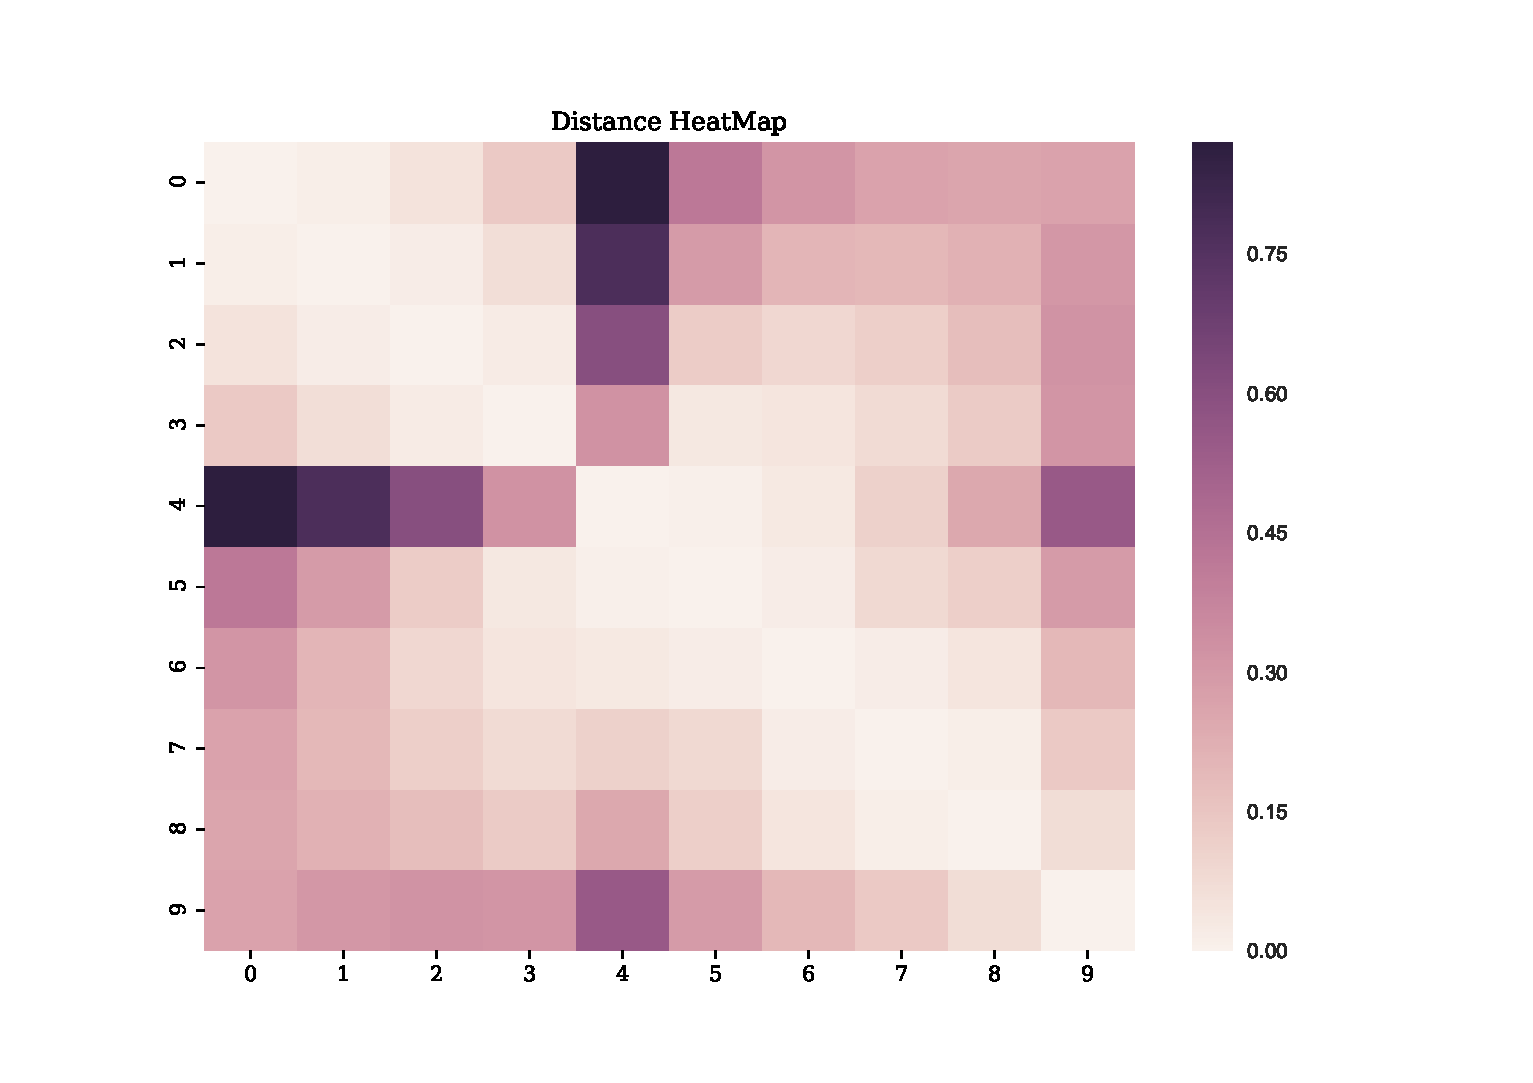
\includegraphics[width=240pt]{figure/fig_sa_heatmap.eps}
  \caption{Hi}
\label{saHeatmap}
\end{figure}

\begin{figure}
\centering
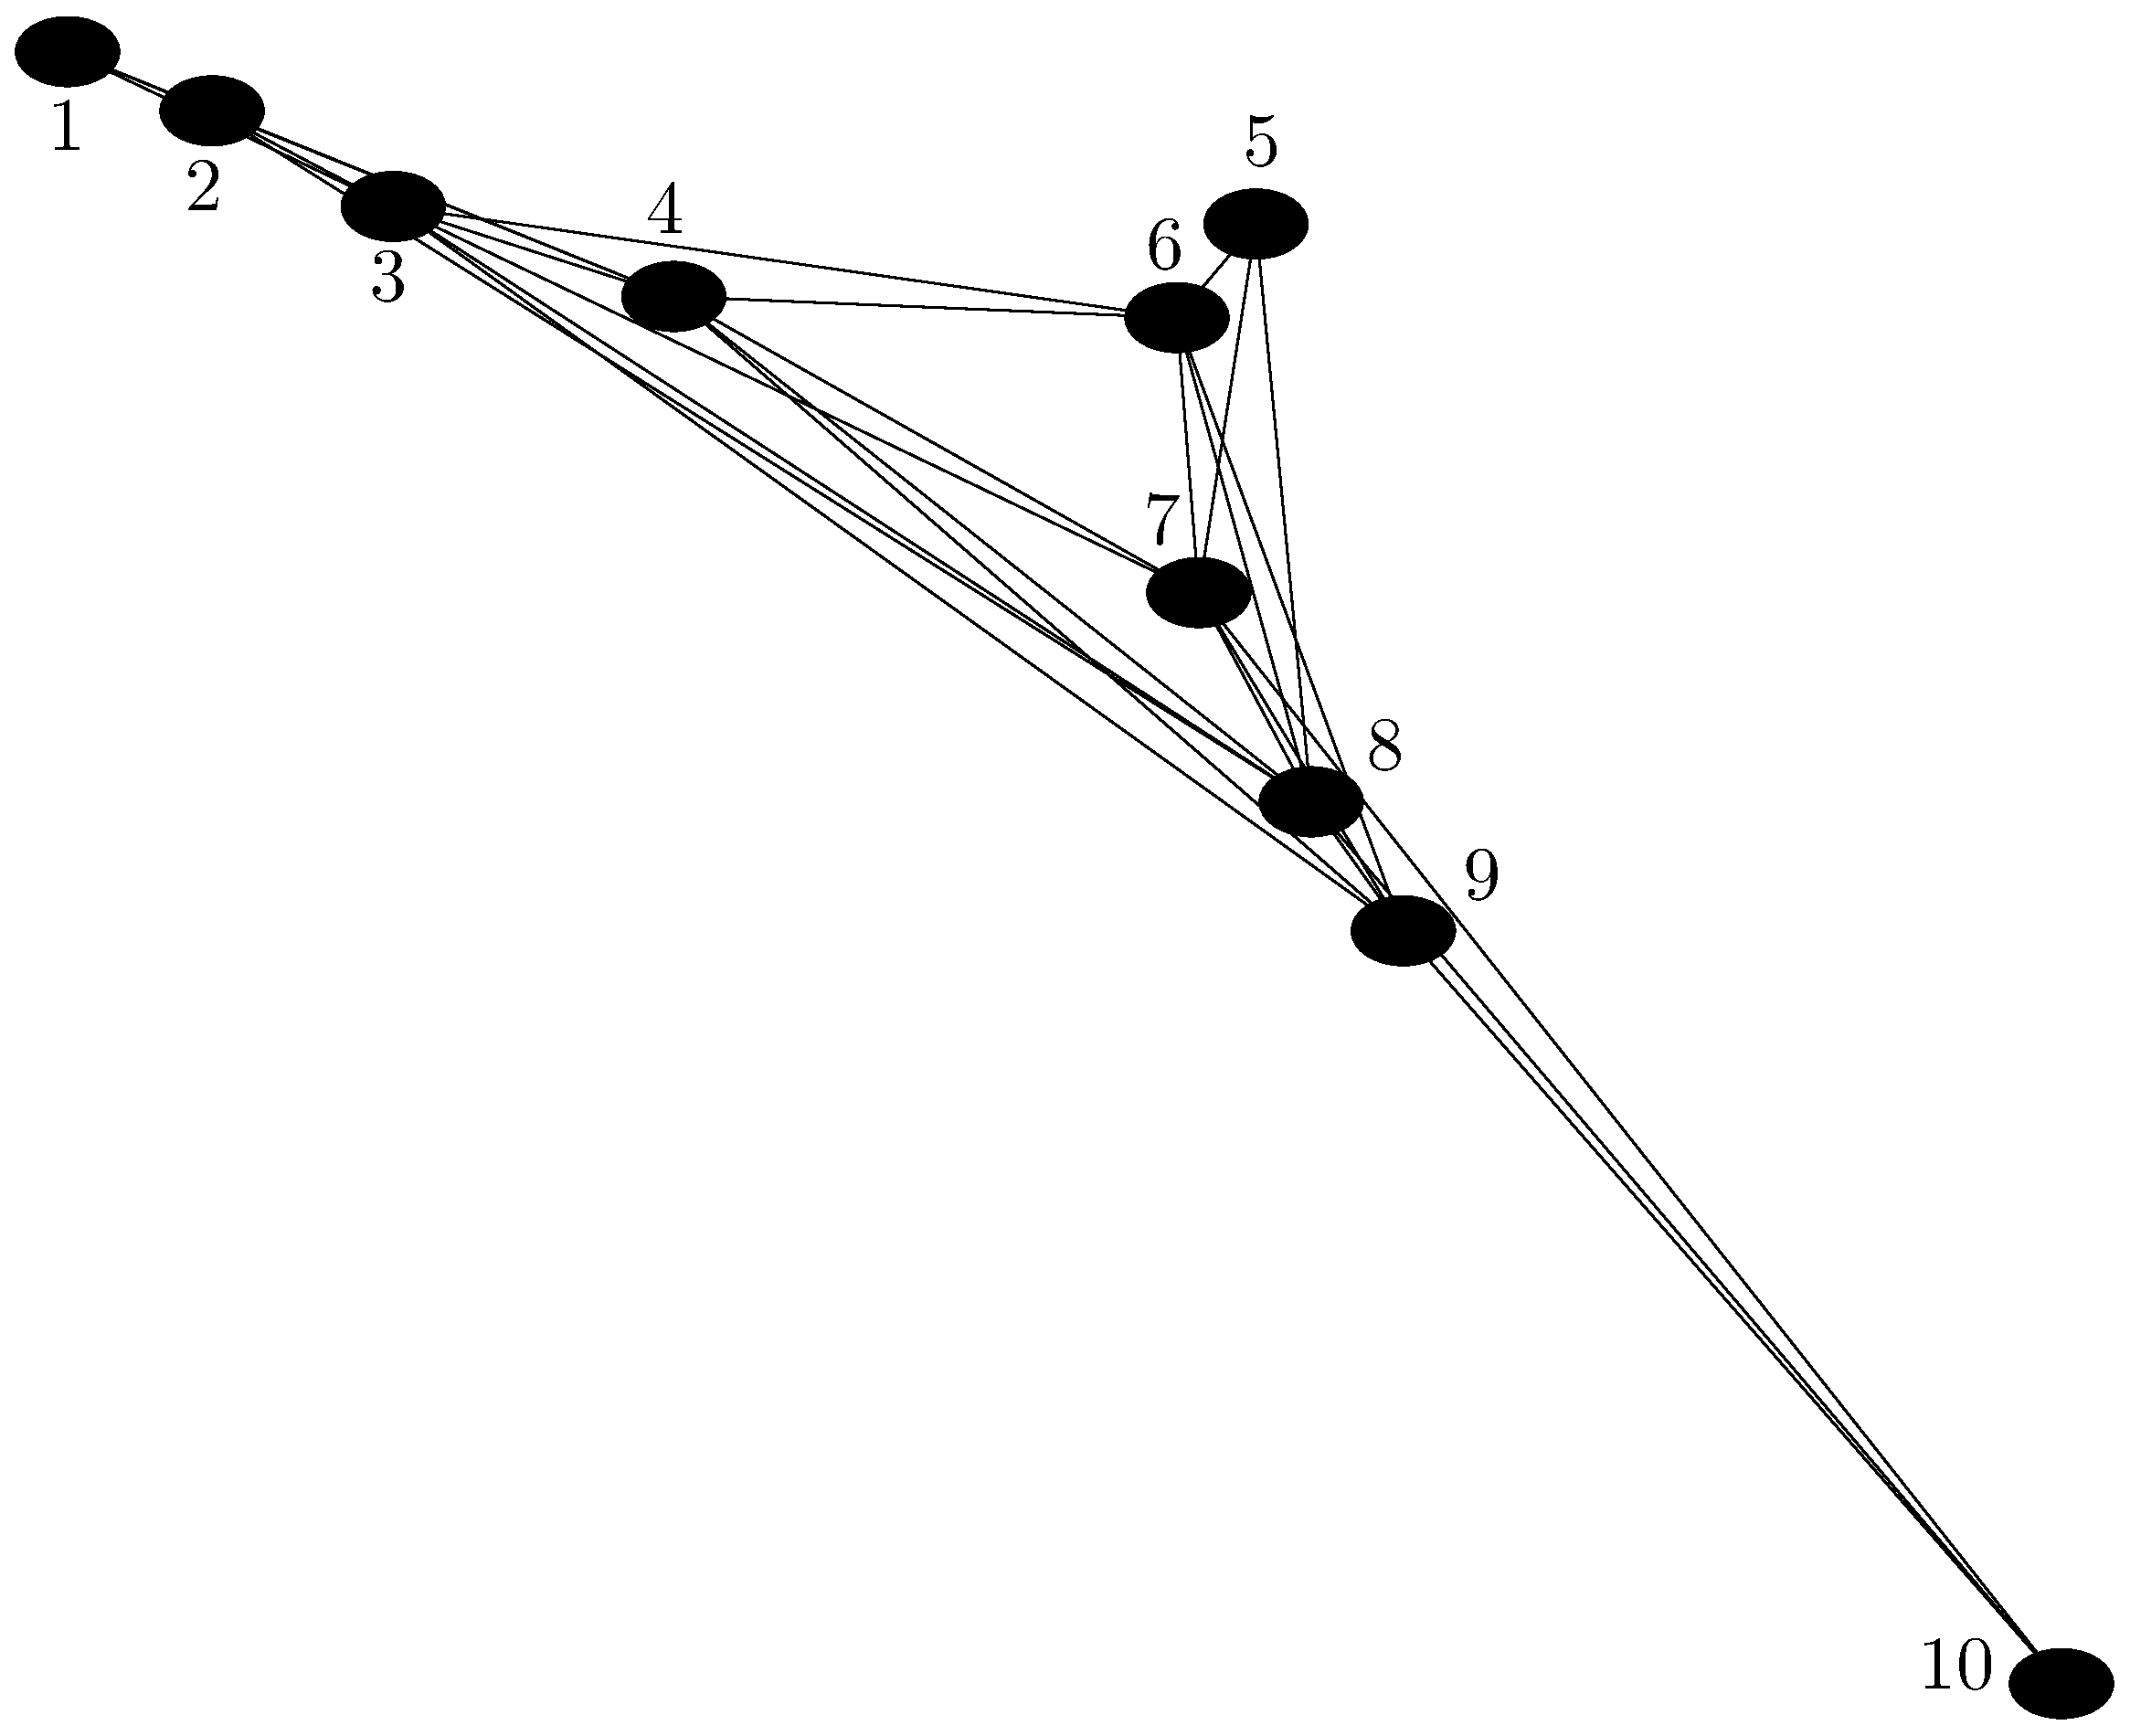
\includegraphics[width=240pt]{figure/fig_sa_graph.eps}
  \caption{Hi}
\label{saGraph}
\end{figure}

\section{Clustered Database of Planar Linkages}
Having a invariant representation greatly reduces data required to sample all possible types shapes of coupler motion.
We have built a database of planar four-bar linkages with revolute joints as an example, but the approach is same for any planar motion generating machine.
We generate this database while taking following aspects into consideration.
\begin{enumerate}
  \item Sampling should maximize its distribution over possible four-bar coupler motions.
  \item Data generation can be parallelized.
  \item Approach scalable with linkages with more number of links.
\end{enumerate}
Figure~\ref{fourbar} represents parametric representation of four-bar linkage with parameters ($l_1,l_2,l_3,l_4,l_5$).
As mapping between four-bar linkage parameter space and coupler motion space is highly non-linear, uniform distribution over linkage parameter space doesn't necessarily mean uniform sampling over motion space.
Thus the efficient approach would be to sample more in the locations where sensitivity is maximum.
Our observational intuition tells that whenever the link ratios of four-bar linkage are close to 1, the sensitivity of the shape of a coupler motion is higher than otherwise.
Thus we chose Log-Normal Distribution ($\mu = 0,\sigma = 0.6 $) for the range of link ratios : $(l_1, l_2, l_3)$ as shown in Fig.~\ref{logNormal}, and Normal Distribution ($\mu = 0,\sigma = 2 $) for $(l_4, l_5)$.

\begin{figure}
\centering
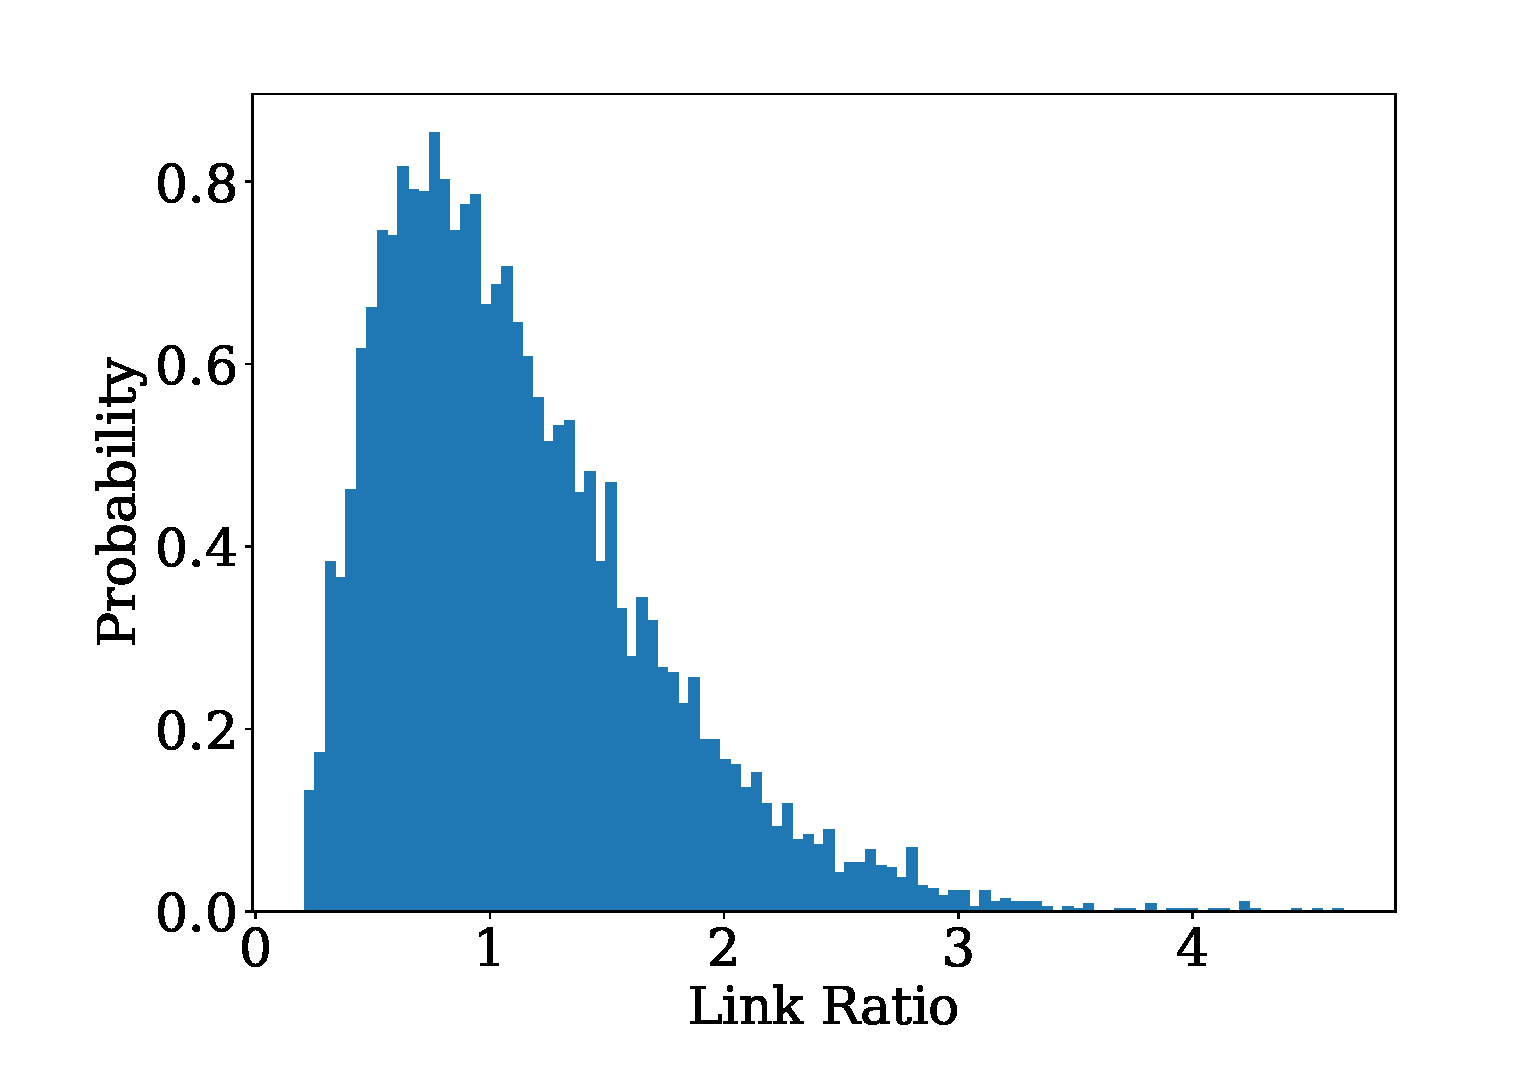
\includegraphics[width=240pt]{figure/fig_logNormal.eps}
  \caption{Probability Distribution function used in random sampling for parameters $l_1$, $l_2$ and $l_3$.}
\label{logNormal}
\end{figure}

\subsection{Dimensionality Reduction using Auto-Encoders}
Each data point in database consists of discrite signature of motion, which is kept to be 100 float digits. In order to have efficient query operations we perform clustering, a method that summarizes and creates a hierarchy in the database.
Clustering in higher dimensions suffers from \emph{Curse of Dimensionality}, thus we first perform dimensionality reduction using Auto-encoder Neural Networks.
Auto-encoder is a powerful mapping model, which learns to encode the input data in very compact representation and can reconstruct the input with minimal error; performing much better than PCA\cite{hinton2006}.
This Non-linear mapping by auto-encoder can greatly improve the representation of data for clustering\cite{song2013}.
Figure~\ref{autoEncoder} shows an architecture similar to the Neural Network we designed for the task.
Number of neurons per layer are (100, 80, 50, 10, 50, 80, 100).
Each hidden layer is activate by Rectified Linear Unit (\emph{ReLU}) activation function.
In $i^{th}$ hidden layer, output of the previous layer $h_(i-1)$ is fed as input to produce output $h_i$ given by,

\begin{eqnarray}\label{nnlayer}
  h_i = ReLU(W_{i}h_{i-1} + b_{i}), \\
  ReLU(x) = max(0, x).
\end{eqnarray}

Where $W_i$ and $b_i$ are weights and bais of $i^{th}$ layer, which are computed in the process of training.
Auto-encoders are trained to reconstruct the input, in this way each layer encodes the input, which is sufficient for the next layers to reconstruct the output.
Objective of the training is to find out set of weights and biases that minimizes the error loss given by,

\begin{equation}\label{nnloss}
  E = \sum_{i=0}^{N} || X_i - \grave{X}_i ||^2
\end{equation}
where $X_i$ is input, $\grave{X}_i$ is reconstructed output and N is number of training examples.

Once a network is trained, Output of the bottle-neck layer $(h_{ib})$ represents the compressed feature space ($Z$).
It can be seen that input information is compressed by a factor of 10, while achieving $95\%$ reconstruction accuracy.
Standard clustering algorithms are performed on this latent space for better clustering\cite{song2013}.
We use Agglomeretive Clustering, a method of Hierarchical clustering, which is an approach to partitioning clustering for identifying groups in the dataset.
It does not require to pre-specify the number of clusters to be generated.
\emph{Ward}\cite{ward1963} Linkage criterion is used for clustering, which minimizes the variance of the clusters being merged.
The distance metric used is the euclidean distance in the latent space.
Although the more accurate distance metric is normalized cross correlation score, it is very expensive to calculate it for entire database.
Signatures with $\mathcal{O}(m)$ points, take $\mathcal{O}(m\log{}m)$ time for each comparisons and there are $\mathcal{O}(N^2)$ number of comparisons to be made for database of $N$ points.
Thus we pick one sample from each cluster and perform Agglomeretive Clustering on this set with normalized cross correlation as the distance metric to form a top cluster.
When user raises one such query, we first find k nearest neighbors in the top cluster, then descend into their neighbors.
Motion with highest similarity score is returned along with its corresponding linkage parameters which are further fine-tuned to match query using optimization.

\begin{figure}
\centering
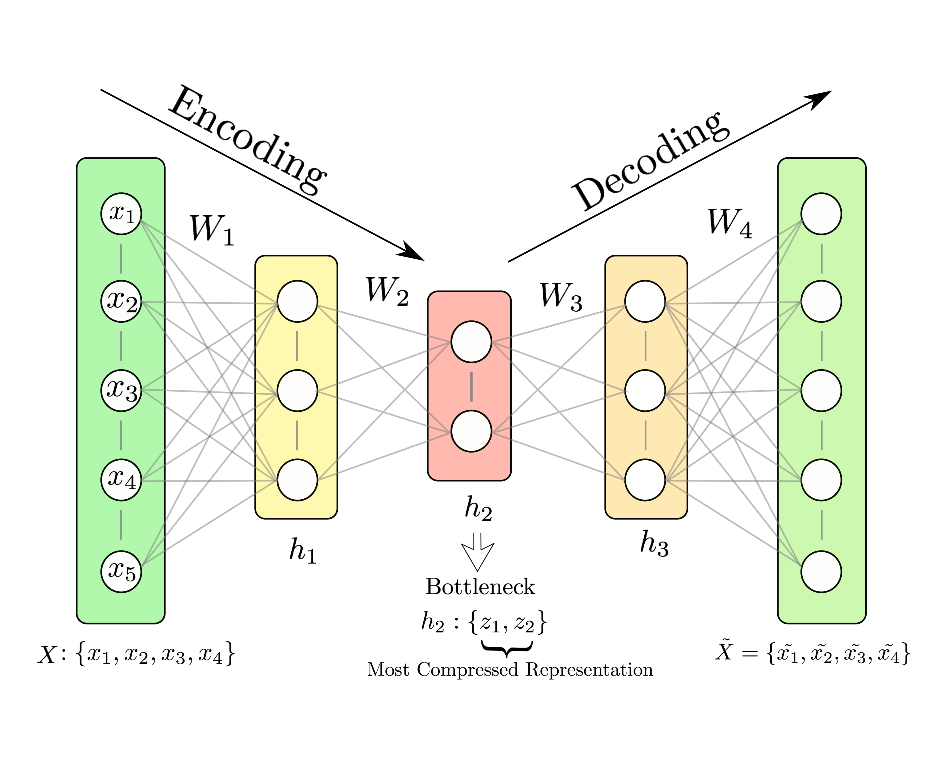
\includegraphics[width=240pt]{figure/fig_auto_encoder.eps}
  \caption{A general architecture of Auto-Encoder. Actual implementation has five hidden layers where middle layer is the bottleneck.}
\label{autoEncoder}
\end{figure}


\section{Algorithm}
\begin{algorithm}[thb]
\caption{Algorithm for Optimal Four-bar Linkage Synthesis}\label{algorithm1}
\begin{algorithmic}[1]
\Procedure{Lagrange Multiplier Method}{}\\
linear constraints$ (n) \leq 5$
\For {each linear constraint}
\State{add constraint eq. to [A]}
\EndFor\label{}
\State{perform SVD and pick $n-8$ Singular Vectors}
\State $f = 0$
 \State{error function for each of the relaxed constraint $\rightarrow$ $f_i$}
 \For {each $f_i$}
\State{$f = f + {f_i}^2$}
\EndFor\label{}
\State{form $h_1$ and $h_2$ using Eq.~\ref{h1h2}}
\If{nonlinear constraints exist}
\State{number of non linear constraints =  $m$}
\For {each $m$}
\State{form $h_{(2+m)}$ using Eq.~\ref{nonlinEq} }
\EndFor\label{}
\EndIf\label{}
\State {{\bf Minimize} $f$ subjected to $h_1 = 0$,..,$h_{(2+m)} = 0$, $g \leq 0$ }
\State {Minimize $F$ by Lagrange Multipliers}
\State {$F = -f - \lambda_1h_1 -...-\lambda_{(m+2)}h_{(m+2)} - \mu g$}
\State {Take partial derivatives of $F$ w.r.t. $\alpha_2$,..,$\alpha_{(8-n)}$,$\lambda_1$,..,$\lambda_{(2+m)}$ to form a system of Equations along with Eq.\req{kkt1}},
\State {{\bf Solve} $(9 - n  + m) $ equations}
\State {{\bf Compute} dyad parameters}
\EndProcedure
\end{algorithmic}
\end{algorithm}

%%%%%%%%%%%%%%%%%%%%%%%%%%%%%%%%%%%%%%%%%%%%%%%%%%%%%%%%%%%%%%%%%%%%%%

\section{Examples}\label{examples}

\begin{table}
\caption{Example~\ref{5pos}: Pose Data}
\centering
\label{5posMotion}
\begin{tabular}{cccc}
\hline
Poses & X & Y & $\phi$ (degree)\\
\hline
Pose 1 &  -5.74803 & -0.00787402 & 88.5679 \\
Pose 2 &  -4.12598 & 0.795276 & 2.16642 \\
Pose 3 &  -2.72441 & 1.67717 & 356.968 \\
Pose 4 &   -1.54331 & 0.433071 & 1.03102 \\
Pose 5 &   1.22835 & -0.590551 & 345.624 \\
\hline
\end{tabular}
\end{table}

\begin{table*}[thb]
  \caption{Example \ref{5pos}: Four singular vectors obtained after SVD of the matrix $[A]$ of size $4\times8$.}
  \centering
  \begin{tabular}{ccccccccc}
  \hline
  Dyad Vector &$p_1$&$p_2$&$p_3$&$p_4$&$p_5$&$p_6$&$p_7$&$p_8$\\
    \hline
   $\textbf{p}_1$& -0.01874 & -0.2516 & 0.5174 & -0.3985 & 0.02237 & 0.03616 & 0.4980 & 0.5097\\
$\textbf{p}_2$&0.007703 & 0.4284 & -0.3233 & 0.5047 & -0.02227 & -0.06264 & 0.4823 & 0.4688\\
$\textbf{p}_3$& 0.02871 & 0.08073 & 0.1114 & 0.1484 & -0.0120 & 0.9778 & -0.03979 & 0.01384\\
$\textbf{p}_4$& 0.07561 & -0.1628 & 0.02429 & 0.1901 & 0.9647 & -0.009039 & -0.007750 & 0.01223\\
    \hline
  \end{tabular}
  \label{svectors5pos}
\end{table*}

\begin{table*}[thb]
  \caption{Example \ref{5pos}: Two optimum dyad-vectors obtained as result of optimization}
  \centering
  \begin{tabular}{ccccccccc}
  \hline
  Vector &$p_1$&$p_2$&$p_3$&$p_4$&$p_5$&$p_6$&$p_7$&$p_8$\\
   \hline
$\textbf{s}_1$&0.4175 & 1.025 & 5.818 & 1.388 & 0.8691 & 17.21 & 7.760 & 8.773 \\
$\textbf{s}_2$&0.08080 & 0.007451 & 0.07404 & 0.3656 & 0.9573 & 0.2468 & 0.4554 & 0.4875\\
   \hline
  \end{tabular}
  \label{dyadvectors5pos}
\end{table*}

\begin{figure}
\centering
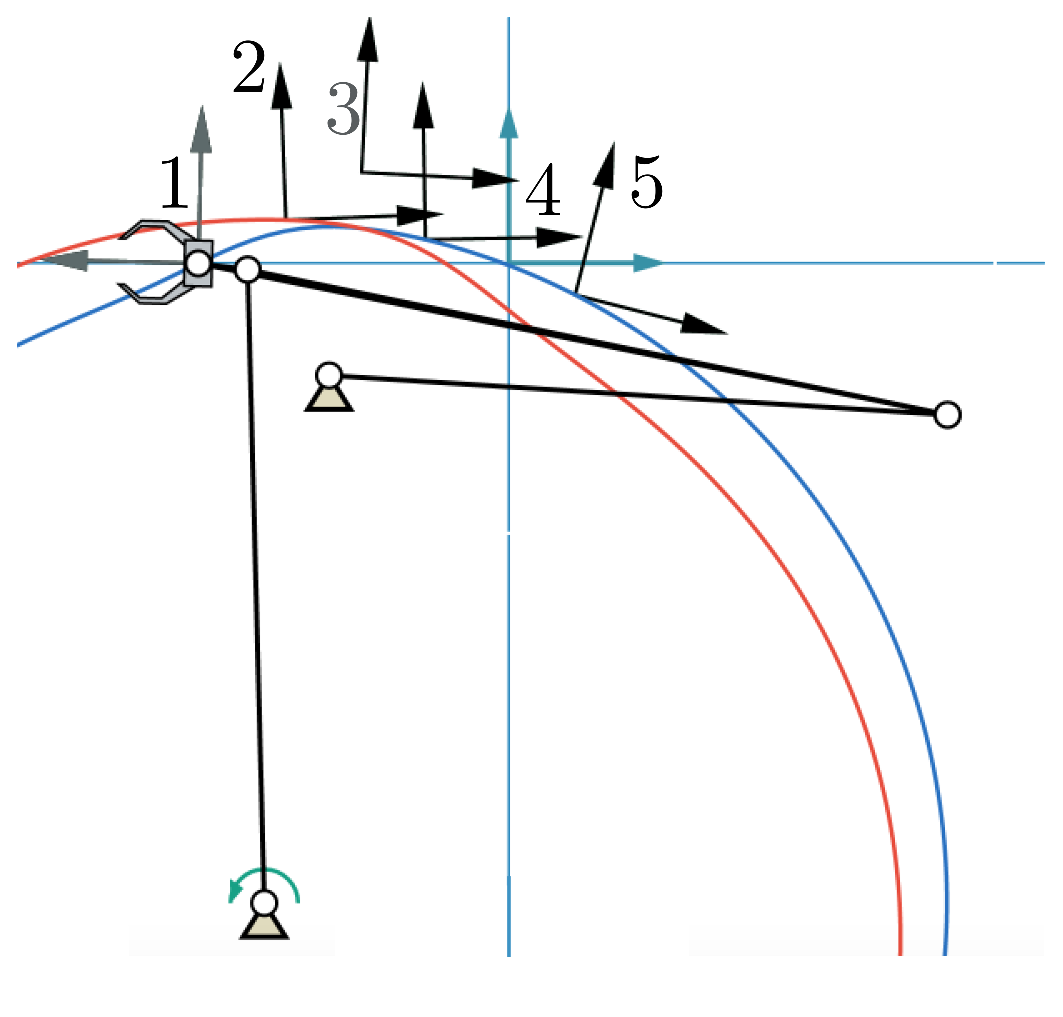
\includegraphics[width=200pt]{figure/fig1.eps}
\caption{Example \ref{5pos}: Optimal four-bar mechanism that minimizes algebraic fitting error for third pose. Although second pose lies on different circuit, this Grashof type four-bar produces desired continuous motion from first to last pose.}
\label{5posgg}
\end{figure}

\subsection{Optimal Linkage for Four Precision Poses with Region Constraint}\label{4pos1line1pose}
\begin{figure}
\centering
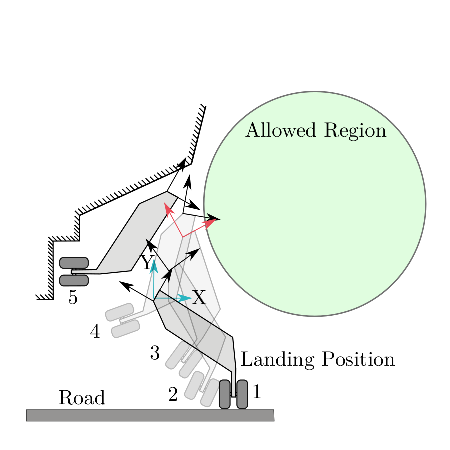
\includegraphics[width=230pt]{figure/fig2.eps}
\caption{Example \ref{4pos1line1pose}: Five landing gear positions are shown where the third position can be relaxed. Allowed region for fixed pivots of mechanism is also shown.}
\label{4posproblem}
\end{figure}

\begin{table}
\caption{Example~\ref{4pos1line1pose}: Pose Data}
\centering
\label{4posMotion}
\begin{tabular}{cccc}
\hline
Poses & X & Y & $\phi$ (degree)\\
\hline
Pose 1 &  -0.0125 & -0.0374 & 66.3 \\
Pose 2 &  0.303 & 0.634 & 35.5 \\
Pose 3 &  0.599 & 1.83 & 352. \\
Pose 4 &  0.268 & 2.30 & 331. \\
Pose 5 &  0.606 & 1.31 & 22.2 \\
\hline
\end{tabular}
\end{table}

\begin{table*}[thb]
  \caption{Example \ref{4pos1line1pose}: Four singular vectors obtained after SVD of the matrix $[A]$ of size $4\times8$. The vectors form basis for the null space}
  \centering
  \begin{tabular}{ccccccccc}
  \hline
  Vector &$p_1$&$p_2$&$p_3$&$p_4$&$p_5$&$p_6$&$p_7$&$p_8$\\
    \hline
   $\textbf{p}_1$& -0.585 & -0.0211 & -0.506 & 0.165 & 0.134 & -0.350 & 0.368 & 0.313 \\
   $\textbf{p}_2$& 0.0640 & -0.330 & 0.190 & -0.804 & 0.236 & -0.264 & 0.194 & 0.204 \\
   $\textbf{p}_3$& -0.280 & 0.0484 & -0.466 & -0.398 & 0.232 & 0.603 & -0.136 & -0.329 \\
   $\textbf{p}_4$& -0.137 & 0.145 & 0.469 & 0.250 & 0.747 & 0.229 & 0.259 & 0.0111 \\
    \hline
  \end{tabular}
  \label{svectors4pos}
\end{table*}

\begin{table*}[thb]
 \caption{Example \ref{4pos1line1pose}: Four optimum dyad-vectors obtained as result of optimization}
  \centering
  \begin{tabular}{ccccccccc}
  \hline
  Vector &$p_1$&$p_2$&$p_3$&$p_4$&$p_5$&$p_6$&$p_7$&$p_8$\\
    \hline
$\textbf{s}_1$&  0.0254 & 0.192 & -0.202 & -0.0965 & 0.00562 & 0.723 & -0.387 & -0.490 \\
$\textbf{s}_2$& 0.276 & -0.406 & 0.211 & -0.425 & -0.161 & -0.561 & 0.251 & 0.360 \\
$\textbf{s}_3$& 0.315 & -0.356 & 0.189 & -0.397 & -0.318 & -0.598 & 0.129 & 0.324 \\
$\textbf{s}_4$& 0.208 & -0.302 & 0.141 & -0.335 & -0.321 & -0.691 & 0.134 & 0.368 \\
    \hline
  \end{tabular}
  \label{dyadvectors4pos}
\end{table*}

Figure~\ref{4posproblem} shows five positions of a landing gear moving from the landing position to the retracted position. Table~\ref{4posMotion} contains position and orientation data for five poses. It is desirable that fixed pivots should lie inside the circle of radius 2.3 with center located at (3.33, 2.04). The task is to synthesize a mechanism which interpolates through precision poses (1,2,4,5) and minimizes the algebraic error for the third pose while keeping fixed pivot locations inside the allowed region as shown in the figure.

First step is to extract all four geometric constraints, i.e. four precision poses and form matrix $[A]$  using Eq.~\req{A8}. Here $n = 4$ which means solution space consists of 4 singular vectors which are obtained using SVD and tabulated in Table~\ref{svectors4pos}. Once this linear algebraic fitting is done, optimization problem can be formulated.

The error function is linear error function $f_1$ for third pose, which is evaluated using Eq.~\req{poseError}. Substituting singular vectors into dyad coefficients followed by substituting them in terms of $\alpha_i$ using Eq.~\req{solutionSpace}, we get final objective function given by
\begin{equation}
f = f_1^2,
\end{equation}
where $f_1 = -0.0598 {\alpha_2}+0.0294 {\alpha_3}-0.100 {\alpha_4}+0.0876$.
The circular region for fixed pivots is modeled as an inequality constraint using Eq.~\req{ellipseIneq} and~\req{g} given by,
\begin{equation}
\begin{array}{c}
g = 0.091 {\alpha_2}^2+(0.25 {\alpha_3}+0.11 {\alpha_4}+0.25) {\alpha_2}\\+0.35 {\alpha_3}^2+0.049 {\alpha_4}^2+{\alpha_3} (0.043 {\alpha_4}+1.0)\\-0.048 {\alpha_4}-0.19 \leq 0
\end{array}
\end{equation}
Objective function also has two quadratic equality constraints given by,
\begin{eqnarray}
& & h_1 = 0.058 {\alpha_2}^2+(-0.25 {\alpha_3}+0.17 {\alpha_4}-0.36) {\alpha_2} -0.34 {\alpha_3}^2  \nonumber \\
& & \ \ \ \ \ \ \ \ \  -0.041 {\alpha_4}^2+{\alpha_3} (0.23 {\alpha_4}-0.38)-0.033 {\alpha_4}+0.29, \nonumber \\
& & h_2  = -0.29 {\alpha_2}^2+{\alpha_2} (-0.15 {\alpha_3}-0.074 {\alpha_4}-0.048)+0.20 {\alpha_3}^2 \nonumber \\
& & \ \ \ \ \ \ \ \ \  +{\alpha_3} (0.18 {\alpha_4}+0.12)-0.46 {\alpha_4}^2-0.11 {\alpha_4}-0.36 \nonumber \\
\end{eqnarray}
We follow steps presented in section~\ref{lagrangeMultiplier} and form Lagrange objective function $F$ given by,
\begin{equation}
F = -{f_1}^2- \lambda_1h_1 -  \lambda_2h_2 - \mu g
\end{equation}
and obtain equations by partial differentiation as well as equation corresponding to Karush-Kuhn-Tucker condition as follow:

\begin{equation}
\begin{array}{c}
\frac{\partial}{\partial \alpha_2}(F) = 0 = (-0.12 {\alpha_2}+0.25 {\alpha_3}-0.17 {\alpha_4}+0.36) {\lambda_1}+(0.57 {\alpha_2}\\+0.15 {\alpha_3}+0.074 {\alpha_4}+0.048) {\lambda_2}-(0.18 {\alpha_2}) \mu \\-(0.25 {\alpha_3}) \mu -(0.11 {\alpha_4}) \mu -0.25 \mu +0.060
\end{array}
\end{equation}

\begin{equation}
\begin{array}{c}
\frac{\partial}{\partial \alpha_3}(F) = 0 = {\lambda_1} (0.25 {\alpha_2}+0.69 {\alpha_3}-0.23 {\alpha_4}+0.38)+{\lambda_2}\\ (0.15 {\alpha_2}-0.41 {\alpha_3}-0.18 {\alpha_4}-0.12)-0.25 {\alpha_2} \mu\\ -0.71 {\alpha_3} \mu -0.043 {\alpha_4} \mu -1.0 \mu -0.029
\end{array}
\end{equation}

\begin{equation}
\begin{array}{c}
\frac{\partial}{\partial \alpha_4}(F) = 0 = {\lambda_1} (-0.17 {\alpha_2}-0.23 {\alpha_3}+0.081 {\alpha_4}+0.033)\\+{\lambda_2} (0.074 {\alpha_2}-0.18 {\alpha_3}+0.92 {\alpha_4}+0.11)-0.11 {\alpha_2} \mu\\ -0.043 {\alpha_3} \mu -0.097 {\alpha_4} \mu +0.048 \mu +0.10
\end{array}
\end{equation}

\begin{equation}
\begin{array}{c}
\frac{\partial}{\partial \lambda_1}(F) = 0 =-0.058 \alpha_2^2+(0.25 \alpha_3-0.17 \alpha_4+0.36) \alpha_2\\+0.34 \alpha_3^2+0.041 \alpha_4^2+\alpha_3 (0.38-0.23 \alpha_4)+0.033 \alpha_4-0.29
\end{array}
\end{equation}

\begin{equation}
\begin{array}{c}
\frac{\partial}{\partial \lambda_2}(F) = 0 =0.29 \alpha_2^2+(0.15 \alpha_3+0.074 \alpha_4+0.048) \alpha_2\\-0.20 \alpha_3^2+0.46 \alpha_4^2+\alpha_3 (-0.18 \alpha_4-0.12)+0.11 \alpha_4+0.36
\end{array}
\end{equation}

\begin{equation}
\begin{array}{c}
\mu\frac{\partial}{\partial \mu}(F) = 0 =\mu(-0.091 \alpha_2^2+(-0.25 \alpha_3-0.11 \alpha_4-0.25) \alpha_2\\-0.35 \alpha_3^2-0.049 \alpha_4^2+\alpha_3 (-0.043 \alpha_4-1.0)+0.048 \alpha_4+0.19)
\end{array}
\end{equation}

Solving these equations followed by filtering on the basis of feasibility using Eq.~\ref{kkt2} yields four unique and feasible solutions tabulated in Table~\ref{alphasol}. All of these solutions satisfy Karush-Kuhn-Tucker Condition for optimality given by Eq.~\req{kkt3}. Dyad vectors are calculated by substituting these solutions into \req{solutionSpace} and are given in Table ~\ref{dyadvectors4pos}. Any of these four dyad-vectors when substituted in Eq.~\req{general} forms a quartic equation, which when projected on hyperplane $Z_4 = 1$ represents a quadric surface. Fig.~\ref{4posmanifolds} shows intersection of hyperboloid and hyperbolic paraboloid  formed from first and second dyad-vectors. The intersection curve represents workspace of the corresponding four-bar linkage. Table~\ref{error4pos} contains the minimized algebraic fitting error of objective function. From this table, we can see that dyad $\textbf{s}_4$ has least pose fitting error. All dyads except $\textbf{s}_1$ are of RR type dyads while $\textbf{s}_1$ is an RP dyad. Figure~\ref{4posRRRP} shows a branch defect free four-bar mechanism formed by combining $\textbf{s}_1$ and $\textbf{s}_2$.

\begin{table}
\caption{Real Solutions for $\alpha_i$, $\lambda_i$ and $\mu$}
\centering
\label{alphasol}
\begin{tabular}{cccccccc}
\hline
Dyad &$\alpha_1$&$\alpha_2$ & $\alpha_3$& $\alpha_4$& $\lambda_1$& $\lambda_2$& $\mu$\\
\hline
$\textbf{s}_1$  & 1 & -0.40 & -0.027 & 1.09 & 0.0 & 0.0 & 0.0 \\
$\textbf{s}_2$ & 1 &  -2.04 & -1.81 & 2.06 & 0.0 & 0.0 & 0.0 \\
$\textbf{s}_3$ & 1 &-3.64 & -4.24 & 5.37 & 0.0 & 0.0 & 0.0 \\
$\textbf{s}_4$ & 1 & 5.08 & -2.58 & -2.94  & 0.0 & 0.0 & 0.0 \\
\hline
\end{tabular}
\end{table}

\begin{table}
\caption{Optimality Evaluations for Dyads}
\centering
\label{error4pos}
\begin{tabular}{ccc}
\hline
Dyad & $3^{rd}$Pose-Fitting Error & Inequality Constraint \\
\hline
$\textbf{s}_1$ &  0.0102 & -0.000650 \\
$\textbf{s}_2$ &  0.0415 & -0.00126 \\
$\textbf{s}_3$ &  0.0212 & -0.000424 \\
$\textbf{s}_4$ & -1.8$\times10^{-8}$ &  -0.396 \\
\hline
\end{tabular}
\end{table}

\begin{figure}
\centering
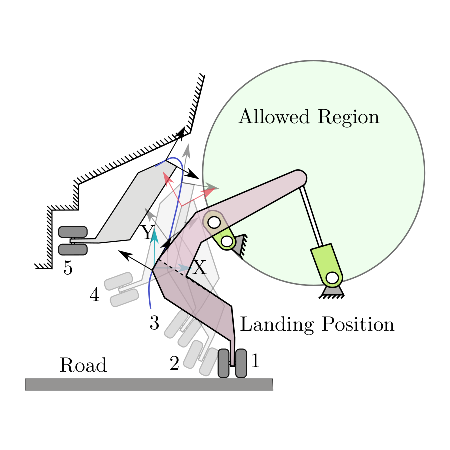
\includegraphics[width=230pt]{figure/fig3.eps}
\caption{Example \ref{4pos1line1pose}: First and second dyad in Table ~\ref{dyadvectors4pos} are combined to form the linkage shown. It can be clearly seen that coupler curve fairly approximates the third pose while fixed pivots are inside the allowed region.}
\label{4posRRRP}
\end{figure}

\begin{figure}
\centering
\includegraphics[width=250pt]{figure/fig4.eps}
\caption{Example \ref{4pos1line1pose}: Image-Space representation of intersection of third and fourth optimal constraint manifolds from Table.~\ref{dyadvectors4pos}. Also shown are five image points as dark spheres representing the five poses; four of them lie exactly on the intersection of the two surfaces, while one is closest possible.}
\label{4posmanifolds}
\end{figure}

\section*{Conclusion}
In this paper, we presented a task-driven approach to unified and optimal synthesis of planar four-bar linkages for extended Burmester problem. In this formulation, various geometric constraints are treated equivalently, which in turn leads to a much simpler two-step based algorithm for computing planar dyads of four-bar linkages. Original contributions of this paper have been into reforming a mixed exact-approximate algebraic fitting problem into problem of task oriented optimal fitting of algebraic manifold. The framework presented here can accommodate linear as well as non-linear equality and inequality geometric constraints and minimize objective functions that can be expressed in terms of dyadic parameters. Although adding non-linear geometric constraints increase computational complexity, computer algebra software like Mathematica could be used to compute solutions of quadratic system of equations in a reasonable amount of time. Experimentations show that Mathematica takes less than 3 seconds on a MacBook Pro with 2.4GHz Intel core i5 processor and 8GB RAM for computing solutions for the system of seven quadratic equations. The framework also preserves previously achieved real-time solutions for linear geometric constraints with no optimality criterion. Two examples demonstrating computation of optimal type and dimensions of dyads that minimize task oriented objective function are presented.

\begin{acknowledgment}
This work has been financially supported by National Science Foundation under a research grant to Stony Brook University (A. Purwar and Q.J. Ge, grant CMMI-1563413). All findings and results presented in this paper are those of the authors and do not represent those of the funding agencies.
\end{acknowledgment}

\bibliographystyle{purwar}
\bibliography{References}
\newpage
\clearpage
\listoftables
\listoffigures

\end{document}
